\subsection{基于图片搜索的神经机器翻译}
\begin{figure}[!htbp]
    \centering
    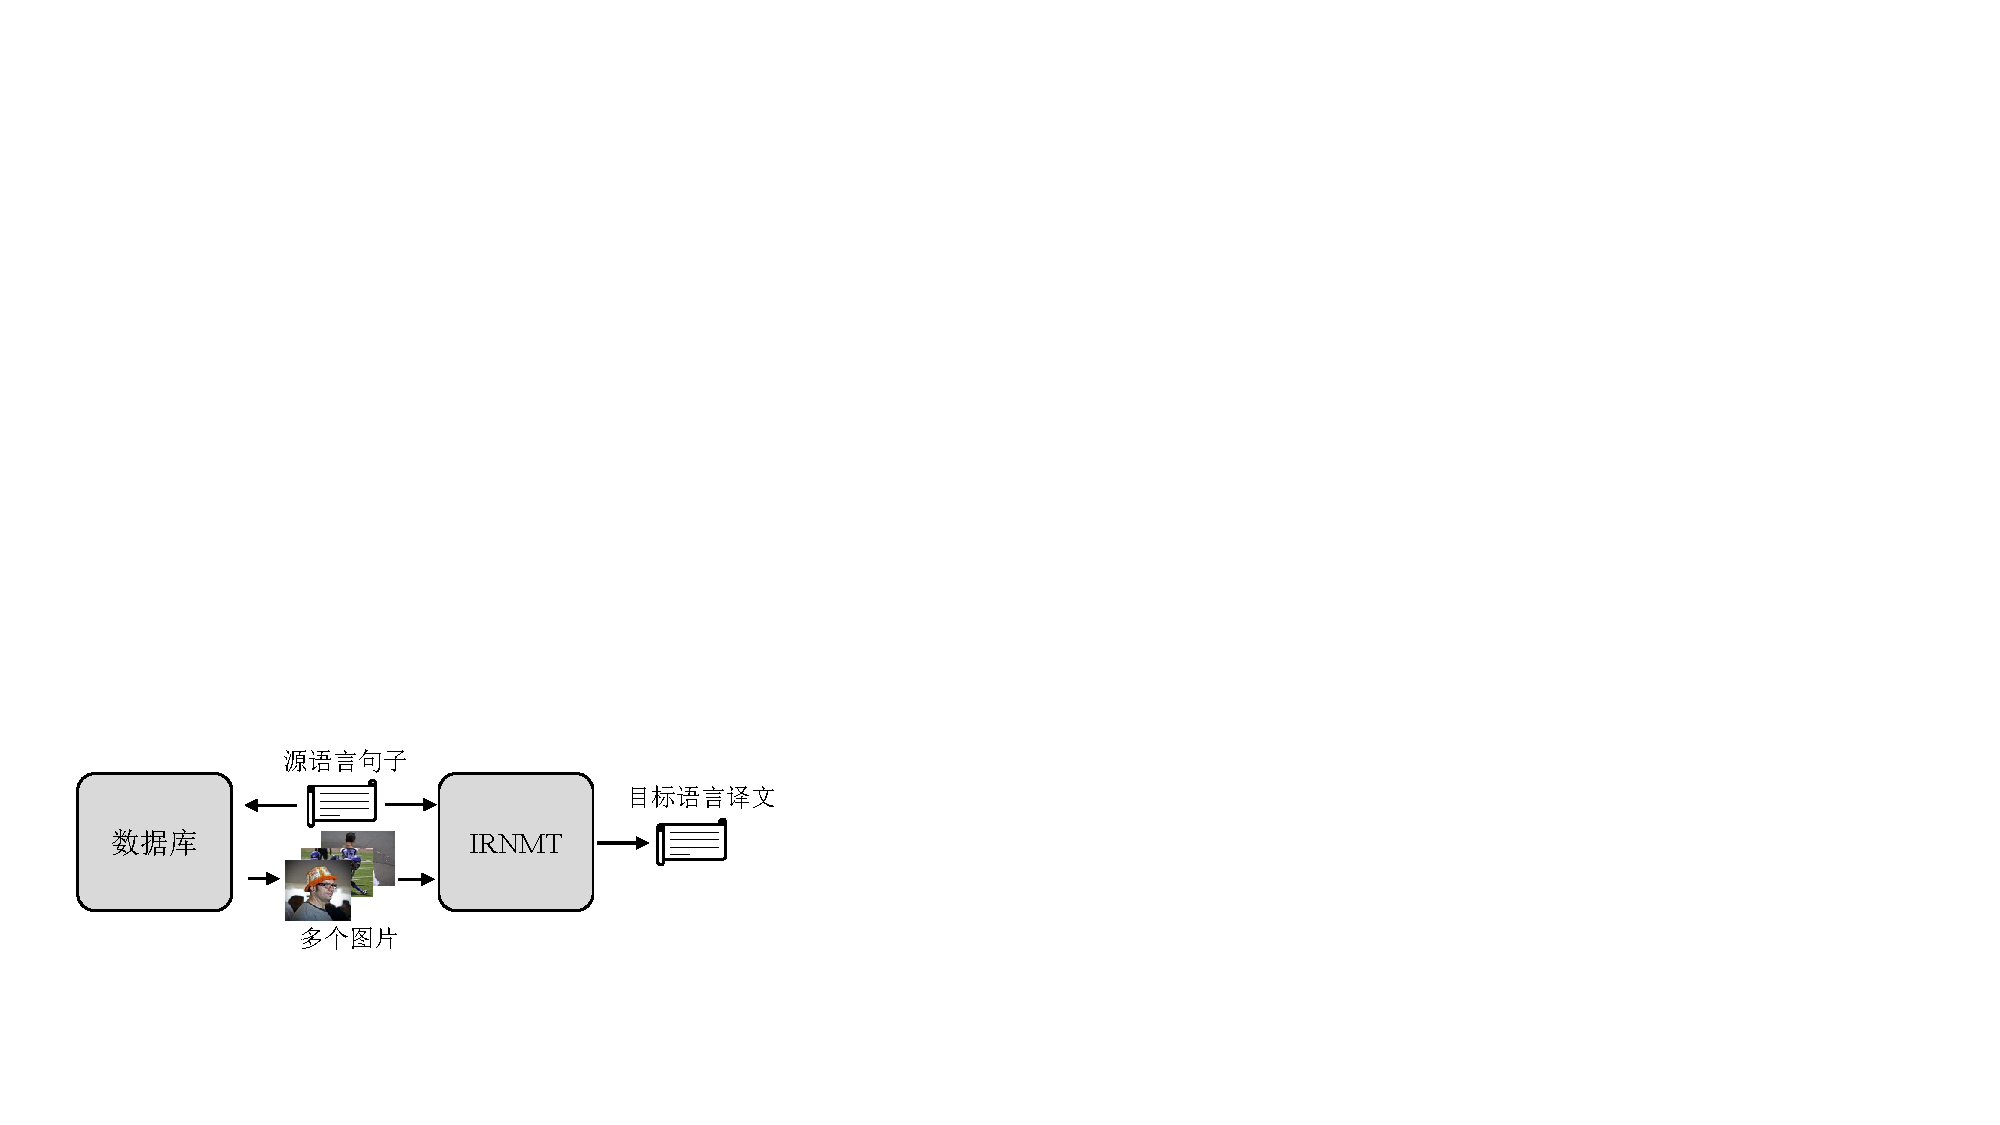
\includegraphics[scale=1]{Img/fig_2_irnmt.pdf}
    \bicaption{基于图片搜索的神经机器翻译}{Image-retrieval-based neural machine translation}
    \label{fig:2_irnmt}
\end{figure}
前两节所介绍的图片信息辅助式和图片信息增强式的神经机器翻译方法采用的都是与文本有着很强语义关系图片。因此,通常在图片描述的翻译任务上进行相关的研究与实验。本节的基于图片搜索的神经机器翻译(image-retrieval-based neural machine translation,IRNMT)与前面的方法区别在于该方法并不要求文本所描述的内容与图片内容完全一致。该方法采用与文本主题相关的搜索方法,从大规模单语语料或搜索引擎中收集相关图片。如图\ref{fig:2_irnmt}所示,为此类方法的研究范式示意图。文献\cite{118_DBLP:conf/iclr/0001C0USLZ20}首次提出在融合图片信息的神经机器翻译模型中增加搜索图片功能。该方法利用TF-IDF(term frequency-inverse document frequency)技术建立一个单词到图片的查找表,从这个查找表中可以获得图片的相关主题信息。在进行图片搜索之前,需要从源语言句子中提取出与句子内容相关的主题单词,然后根据主题搜索出若干个与该主题最相关的图片以此来获得所需要的图片信息。然后将这些图片的特征提取出来,最后传递给神经机器翻译模型用于辅助翻译生成。文献\cite{20_wu-etal-2021-good}在以上基于图片搜索的方法中测试图片信息是否能够为翻译带来提升。文献\cite{119_fang-feng-2022-neural}为了在搜索到更相关的图片,为翻译提供更准确的视觉信息,采用短语级别的图片作用方式,在搜索到图片后,需要提取出与主题相关的视觉目标,然后再进一步地在翻译中融合图片信息。
文献\cite{120_tang-etal-2022-multimodal}为了增加图片搜索的资源,并且使相关方法能够受益于一般的文本翻译任务,采用了基于商用搜索引擎的方案。

目前基于图片搜索的神经机器翻译方法的相关研究还处在初步阶段,基于搜索的方法的相关研究也在问答系统\cite{121_DBLP:conf/icml/GuuLTPC20}、对话系统\cite{122_DBLP:conf/emnlp/WestonDM18}、语言模型\cite{123_DBLP:conf/iclr/KhandelwalLJZL20}以及纯文本翻译\cite{124_DBLP:conf/aaai/GuWCL18}等任务中得到了应用。然而这类方法还存在着诸多问题需要进一步地解决,例如文本主题提取的准确性与覆盖性对图片搜索的影响,搜索获得图片与文本翻译内容的相关性对翻译带来的影响。
%这部分要强调使用完全对应图片的方案都很难使视觉信息起作用,那么采用搜索式的方式就更难了
%方法范式:与前面方法的最大不同点是否图文对应
%举例
%优点
%缺点